% !TEX program = xelatex
\documentclass[a4paper]{article}
\usepackage{amsthm}
\usepackage{amssymb}
\usepackage{bm}
\usepackage{mathtools}
\usepackage[x11names]{xcolor}
\usepackage{xparse}
\usepackage{fontspec}
\usepackage{unicode-math}
\setromanfont{DovesType-Regular.otf}
\setsansfont{Andika}
\setmathfont{Asana Math}[Scale=1]

% \usepackage{pstricks}
\usepackage{varwidth}
\usepackage{siunitx}
\usepackage{graphicx}
\usepackage[margin=1.5cm,top=1.5cm]{geometry}
\usepackage[most]{tcolorbox}
\usepackage{pgfplots}
\pgfplotsset{compat=newest}
\tcbuselibrary{skins,xparse,poster,breakable}
% \usetikzlibrary{fadings}
\usetikzlibrary{calc,math, plotmarks, shapes, shapes.geometric, positioning, angles, intersections, quotes, through, patterns, turtle, arrows.meta}
\usetikzlibrary{decorations.markings,backgrounds}
% \usepackage{etoolbox}
\usepackage{tkz-euclide}
% \usepackage{xlop}
% \newcommand\hole[2]{#1}  % for use with xlop
\pagenumbering{gobble}
%%%%%%%%%%%%%%%%%%%%%%%%%%%%%%%%%%%%%%%%%%%%%%%%%%%%%%%%%
\newcommand\markangle[9]{% origin X Y radius radiusmark mark colour opacity
%  % fill red circle offset-from-centre
  \begin{scope}
    \path[clip] (#1) -- (#2) -- (#3);
    \fill[color=#7,fill opacity=#8,draw=black,name path global=pcircle]  % global declaration required otherwise pcircle is not seen by the `named intersections=' lines below.
    (#1) circle (#4);
  \end{scope}
  % middle calculation
  \path[name path=line one] (#1) -- (#2);
  \path[name path=line two] (#1) -- (#3);
  \path[%
  name intersections={of=line one and pcircle, by={inter one}},
  name intersections={of=line two and pcircle, by={inter two}}
  ] (inter one) -- (inter two) coordinate[pos=#9] (place);
  % put mark
  \node at ($(#1)!#5!(place)$) {\scriptsize{#6}};
}

\newcommand\tcircle[6]{% centre coord (x,y), radius, points, radpoint, colour, edge
  \coordinate (O) at (#1,#2); % centre of the circle
  \def\radius{#3}          % radius of the circle
  \def\npts{#4}            % number of the points
  \def\radpt{#5}           % radius of the points
  \colorlet{ptcolour}{#6}  % colour of the points
  % \draw (O) circle (\radius);
  \foreach \numpoint in {1,...,\npts}{
    \fill[ptcolour] (O) ++ (360/\npts*\numpoint:\radius) coordinate (C\numpoint) circle(\radpt);
  }
}

% \newcommand{\condSoln}[2]{\ifcsdef{r@#1}{#2}{}}

% \newcommand\fadingtext[3][]{%
%    \begin{tikzfadingfrompicture}[name=fading letter]
%      \node[text=transparent!0,inner xsep=0pt,outer xsep=0pt,#1] {#3};
%    \end{tikzfadingfrompicture}%
%    \begin{tikzpicture}[baseline=(textnode.base)]
%      \node[inner sep=0pt,outer sep=0pt,#1](textnode){\phantom{#3}};
%      \shade[path fading=fading letter,#2,fit fading=false]
%      (textnode.south west) rectangle (textnode.north east);%
%    \end{tikzpicture}%
% }

\definecolor{JISpurple}{RGB}{89,72,122}
\definecolor{JISivory}{RGB}{241,234,221}
\definecolor{JIStaupe}{RGB}{183,156,154}
\definecolor{PaleGreen}{RGB}{240,255,240} % 'Honeydew'

\AddToHook{shipout/background}{%
    \put (0in,-\paperheight){
\includegraphics[width=\paperwidth,height=\paperheight]{images/R10V5-R.png}}%
}

\newcommand\numberthis{\addtocounter{equation}{1}\tag{\theequation}}

\newtcolorbox{MyOuterBox}{%
  enhanced,
  % watermark graphics=images/santa_faces_watermark.jpg,
  % watermark opacity=0.8,
  % watermark zoom=2.0,
  breakable,
  frame style=JISpurple,
  colback=JISivory,
  colframe=JISpurple,
  title={
\includegraphics[width=0.9cm,height=0.9cm]{images/JIS Final Logo FA-02.png}\raisebox{3mm}{\Large{Maths Challenge}\hspace{24em} \Large{\bfseries\sffamily 16}}},
}

\newtcolorbox{MyInnerBox}[2][]{enhanced,%empty,
coltitle=JISpurple,colback=white,
breakable,
fonttitle=\bfseries\sffamily,
attach boxed title to top left={yshift=-1.5mm},
boxed title style={empty, size=small, top=1mm, bottom=0pt},
varwidth boxed title=0.5\linewidth,
frame code={
  \path (title.east|-frame.north) coordinate (aux);
\path[draw=JISpurple, line width=0.5mm, rounded corners,fill=white]
(frame.west) |- ([xshift=-2.5mm]title.north east) to[out=0, in=180] ([xshift=7.5mm]aux)-|(frame.east)|-(frame.south)-|cycle;
},
title={#2},#1}

\newtcolorbox{MyInnerSplitBox}[2][]{enhanced,%empty,
bicolor,sidebyside,sidebyside align=top seam,
righthand width=7.5cm,colbacklower=white,
sidebyside gap=5mm,
breakable,
coltitle=JISpurple,colback=white,
fonttitle=\bfseries\sffamily,
attach boxed title to top left={yshift=-1.5mm},
boxed title style={empty, size=small, top=1mm, bottom=0pt},
varwidth boxed title=0.5\linewidth,
frame code={
  \path (title.east|-frame.north) coordinate (aux);
\path[draw=JISpurple, line width=0.5mm, rounded corners,fill=white]
(frame.west) |- ([xshift=-2.5mm]title.north east) to[out=0, in=180] ([xshift=7.5mm]aux)-|(frame.east)|-(frame.south)-|cycle;
},
title={#2},#1}


\newtcolorbox{MySolutionBox}[1][]{%
  enhanced,
  breakable,
  frame style=JISpurple,
  colback=PaleGreen, colframe=green,
  title={\Large Solution},
  drop fuzzy shadow,
  halign=left,
  #1
}

%%%%%%%%%%%%%%%%%%%%%%%%%%%%%%%%%%%%%%%%%%%%%%%%%%
\newtoggle{SOLUTION}
%%% Uncomment the appropriate line below to show solutions %%%
\toggletrue{SOLUTION}
% \togglefalse{SOLUTION}
%%%%%%%%%%%%%%%%%%%%%%%%%%%%%%%%%%%%%%%%%%%%%%%%%


%%%%%%%%%%%%%%%%%%%%%%%%%%%%%%%%%%%%%%%%%%%%%%%%%%
%%%%%%            DOCUMENT BEGINS           %%%%%%
%%%%%%%%%%%%%%%%%%%%%%%%%%%%%%%%%%%%%%%%%%%%%%%%%%
\begin{document}


  \begin{MyOuterBox}
    \iftoggle{SOLUTION}{Here are the full, or partial solutions.
    }{
      Welcome to this week's Maths Challenge!\\
      Have a go at both questions!\\
      Drop your solution in the box in the staffroom by Tuesday.
    }
       \begin{MyInnerBox}{Year 8 and below}
     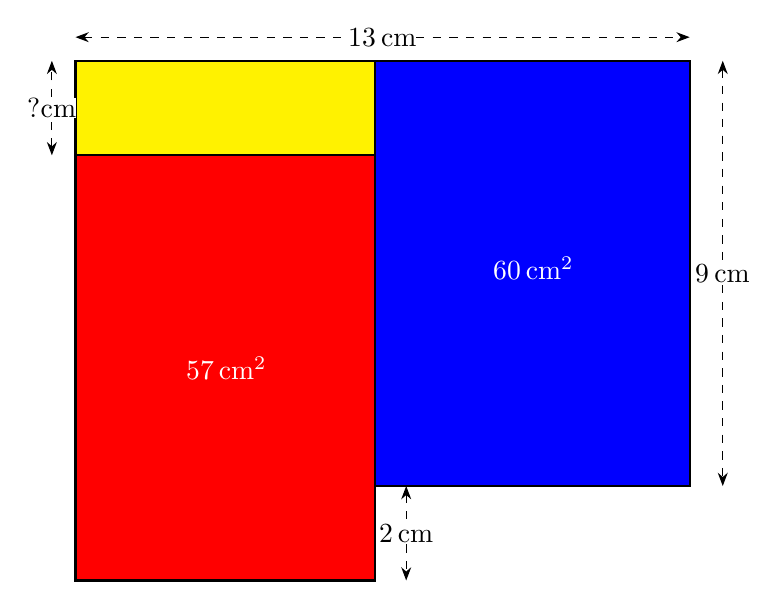
\begin{tikzpicture}[scale=0.6]
       \coordinate (A) at (0,0);
       \coordinate (B) at (0,9);
       \coordinate (C) at (0,11);
       \coordinate (D) at ({19/3},11);
       \coordinate (E) at (13,11);
       \coordinate (F) at (13,2);
       \coordinate (G) at ({19/3},2);
       \coordinate (H) at ({19/3},0);
       \coordinate (I) at ({19/3},9);
       \draw[thick,fill=red] (A) -- (B) -- (I) -- (H) -- cycle;
       \draw[thick,fill=yellow] (B) -- (I) -- (D) -- (C) -- cycle;
       \draw[thick,fill=blue] (G) -- (F) -- (E) -- (D) -- cycle;
       \draw[dashed,Stealth-Stealth] (0,11.5) -- (13,11.5) node[midway,inner sep=0mm,fill=white] {\(\SI{13}{\cm}\)};
       \draw[dashed,Stealth-Stealth] (13.7,11) -- (13.7,2) node[midway,inner sep=0mm,fill=white] {\(\SI{9}{\cm}\)};
       \draw[dashed,Stealth-Stealth] ({21/3},2) -- ({21/3},0) node[midway,inner sep=0mm,fill=white] {\(\SI{2}{\cm}\)};
       \draw[dashed,Stealth-Stealth] (-0.5,9) -- (-0.5,11) node[midway,inner sep=0mm,fill=white] {\(?\SI{}{\cm}\)};
       \node[white] at (3.2,4.5) {\(\SI{57}{\square\cm}\)};
       \node[white] at (9.7,6.6) {\(\SI{60}{\square\cm}\)};
     \end{tikzpicture}
      \iftoggle{SOLUTION}{%conditional output begin
      \begin{MySolutionBox}
        We know the height of the blue rectangle and its area, so we can work out its width.\par
        Width of blue rectangle: \(\frac{60}{9} = \frac{20}{3}\)\par
        So the width of the red and yellow rectangles must be \(13-\frac{20}{3}=\frac{19}{3}\)\par
        As the area of the red rectangle is \(\SI{57}{\square\cm}\), its height must be:\par
        \(57\div\frac{19}{3}=57\times\frac{3}{19}=9\)\par
        Since the total height of the yellow and red rectangles is \(\SI{11}{\cm}\),\par
        the yellow rectangle must be \(\SI{2}{\cm}\) high.
      \end{MySolutionBox}
    }{}%conditional output end
    \end{MyInnerBox}


    \vspace{0.4cm}
          \begin{MyInnerSplitBox}{Year 9 and above}
        Find the value of the shaded angle in the circle in the triangle in the semi-circle. You need to know some basic circle theorems for this.\par
      \iftoggle{SOLUTION}{%conditional output begin
      \begin{MySolutionBox}
        We add some labels to help: \(I\) is the centre of the circle.\par
        Since we are told the shape is a semi-circle, \(PQ\) is a diameter.\par
        So the angle subtended by lines from \(P\) and \(Q\) to the circumference must be \(\SI{90}{\degree}\).\par
        This is a special case of the theorem that says that the angle subtended at the centre of a circle (\(2\phi\)) by two points (\(A\) and \(B\)) on the circumference is double the angle the same two points subtend at the circumference (\(\phi\)). See the diagram below. In this case \(2\phi=\SI{180}{\degree}\) at the centre \(O\), so at the circumference (at \(R\)), the angle is half this.\par
        That is, \(\angle PRQ = \SI{90}{\degree}\)\par
        The circle inside \(\bigtriangleup PQR\) is called the 'incircle' of the triangle. The sides of the triangle \(PQR\) are tangent to the circle at \(L\), \(M\) and \(N\).\par
        A radius of the circle meets a tangent line at right-angles, at the point of tangency.\par
        That is, \(\angle IMR = \angle INR = \SI{90}{\degree}\).\par
        Therefore \(\angle MIN = \SI{90}{\degree}\).\par
        We use the same theorem again: Points \(M\) and \(N\) on the circumference of the circle subtend an angle of \(\SI{90}{\degree}\) at the centre \(I\) of the circle.\par
        So the angle that points \(M\) and \(N\) subtend on the circumference of the circle at point \(L\) must be half that.\par
        The value of the yellow-shaded angle is \(\SI{45}{\degree}\).
      \end{MySolutionBox}
    }{}%conditional output end
        \tcblower
        \begin{tikzpicture}[scale=1.1]
          \def\Rad{3}
          \coordinate (P) at (-\Rad,0);
          \coordinate (R) at (60:\Rad);
          \coordinate (Q) at (\Rad,0);
          \tkzDefCircle[in](P,R,Q)\tkzGetPoint{I}\tkzGetLength{rI}
          \draw (I) circle [radius=\rI];
          \draw (P) -- (Q) node(xline) {} arc(0:180:\Rad) -- cycle;
          \draw[line join=bevel] (P) -- (60:\Rad) coordinate (R) -- (Q);
          \coordinate (M) at ($(R)!\rI cm!(P)$);
          \coordinate (N) at ($(R)!\rI cm!(Q)$);
          \path[] (I) -- (I |- xline) coordinate (L);
          \markangle{L}{M}{N}{5mm}{6mm}{}{yellow}{1}{1}
          \draw[blue,line join=bevel] (M) -- (N) -- (L) -- cycle;
          \iftoggle{SOLUTION}{
            \node[below left] at (P) {\(P\)};
            \node[below right] at (Q) {\(Q\)};
            \node[above] at (R) {\(R\)};
            \node[below] (O) at (0,0) {\(O\)};
            \node[below] at (L) {\(_L\)};
            \node[right] at (N) {\(_N\)};
            \node[above] at (M) {\(_M\)};
            \node[below right=-1mm] at (I) {\(_I\)};
            \draw[dashed] (M) -- (I) (N) -- (I) (L) -- (I);
            \tkzMarkRightAngle[draw=red,fill=red,size=0.15](P,R,Q);
            \tkzMarkRightAngle[draw=red,fill=red,size=0.15](R,M,I);
            \tkzMarkRightAngle[draw=red,fill=red,size=0.15](I,N,R);
            \tkzMarkRightAngle[draw=red,fill=red,size=0.15](M,I,N);
            \draw[blue,line join=bevel] (M) -- (N) -- (L) -- cycle;
            % \filldraw (I) circle (1pt);
          }{}
        \end{tikzpicture}\par\vspace{10mm}\hspace{3em}
        \iftoggle{SOLUTION}{
        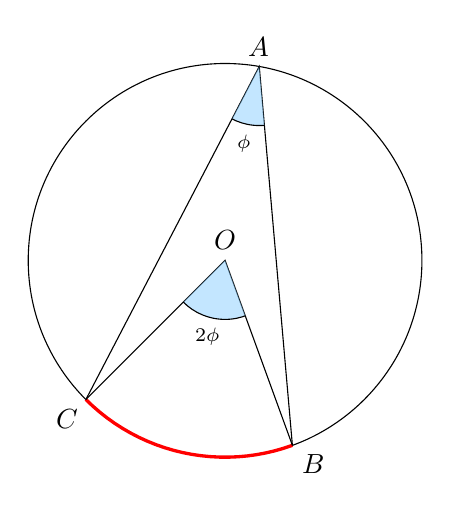
\begin{tikzpicture}[scale=2.5]
          \coordinate [label=above: $O$] (O) at (0,0);
          \node[draw, name path=ci] (ci) at (O) [circle through=(right:1)]{};
          \coordinate [label=below left: $C$] (P) at (ci.225);
          \coordinate [label=below right: $B$] (Q) at (ci.290);
          \draw[red,very thick,domain=225:290] plot({cos(\x)},{sin(\x)});
          \coordinate [label=above: $A$] (A) at (ci.80);
          \draw (P) -- (O) -- (Q);
          \draw (P) -- (A) -- (Q);
          \markangle{O}{P}{Q}{3mm}{4mm}{$2\phi$}{SkyBlue1}{0.5}{0.5};
          \markangle{A}{P}{Q}{3mm}{4mm}{$\phi$}{SkyBlue1}{0.5}{0.5};
      \end{tikzpicture}
    }{}
    \end{MyInnerSplitBox}


  \end{MyOuterBox}

%%%%%%%%%%%%%%%%%%%%%%%%%%%%%%%%%%%%%%%%%%%%%%%%%%
\end{document}



